\documentclass[12pt]{article}
\usepackage[margin=1in,letterpaper]{geometry}
\usepackage{amsmath}
\usepackage{amsfonts}
\usepackage[titletoc,title]{appendix}
\usepackage{graphicx}
\usepackage{hyperref}
\hypersetup{
    colorlinks = true,
    citecolor={black},
    linkcolor={red}
}
\usepackage{titling}
\posttitle{\par\end{center}}
\setlength{\droptitle}{0pt}
\begin{document}
\title{Crowd Segmentation Progress}
\author{\today}
\date{}
\vspace{-50pt}
\maketitle
\vspace{-70pt}
\section{Problem Formulation}
 The goal of quality evaluation is two-folds. Given N worker responses, find: 
 \begin{enumerate}
\item the quality of the bounding boxes (BB) drawn by worker 
\item the best proposed region for a given object in an image
 \end{enumerate}
\section{Key Assumptions and Intuitions}
\begin{enumerate}
\item In literature, there are scoring functions that require ``ground truth" and ones that are ``unsupervised". 
\item If a worker's response differs greatly from the ground truth, then work quality ($Q_w$) is low. 
\item If most of the workers' response differ greatly from ground truth for a particular image, then task difficulty ($D_t$) should be high. As a corollary, if the spread of the $J_i$ distribution is large, then $D_t$ should also be high.
\end{enumerate}
To compute the latent quantities $Q_w$,$D_t$, we propose an iterative EM-like algorithm, where at every step, we assume that the ground truth bounding box ($BB_G$) is the current estimate of the maximum likelihood region. The maximum likelihood region is constructed by adding in sub-regions from a tile-graph. 
\section{Generative Process}
\begin{figure}[ht]
\centering
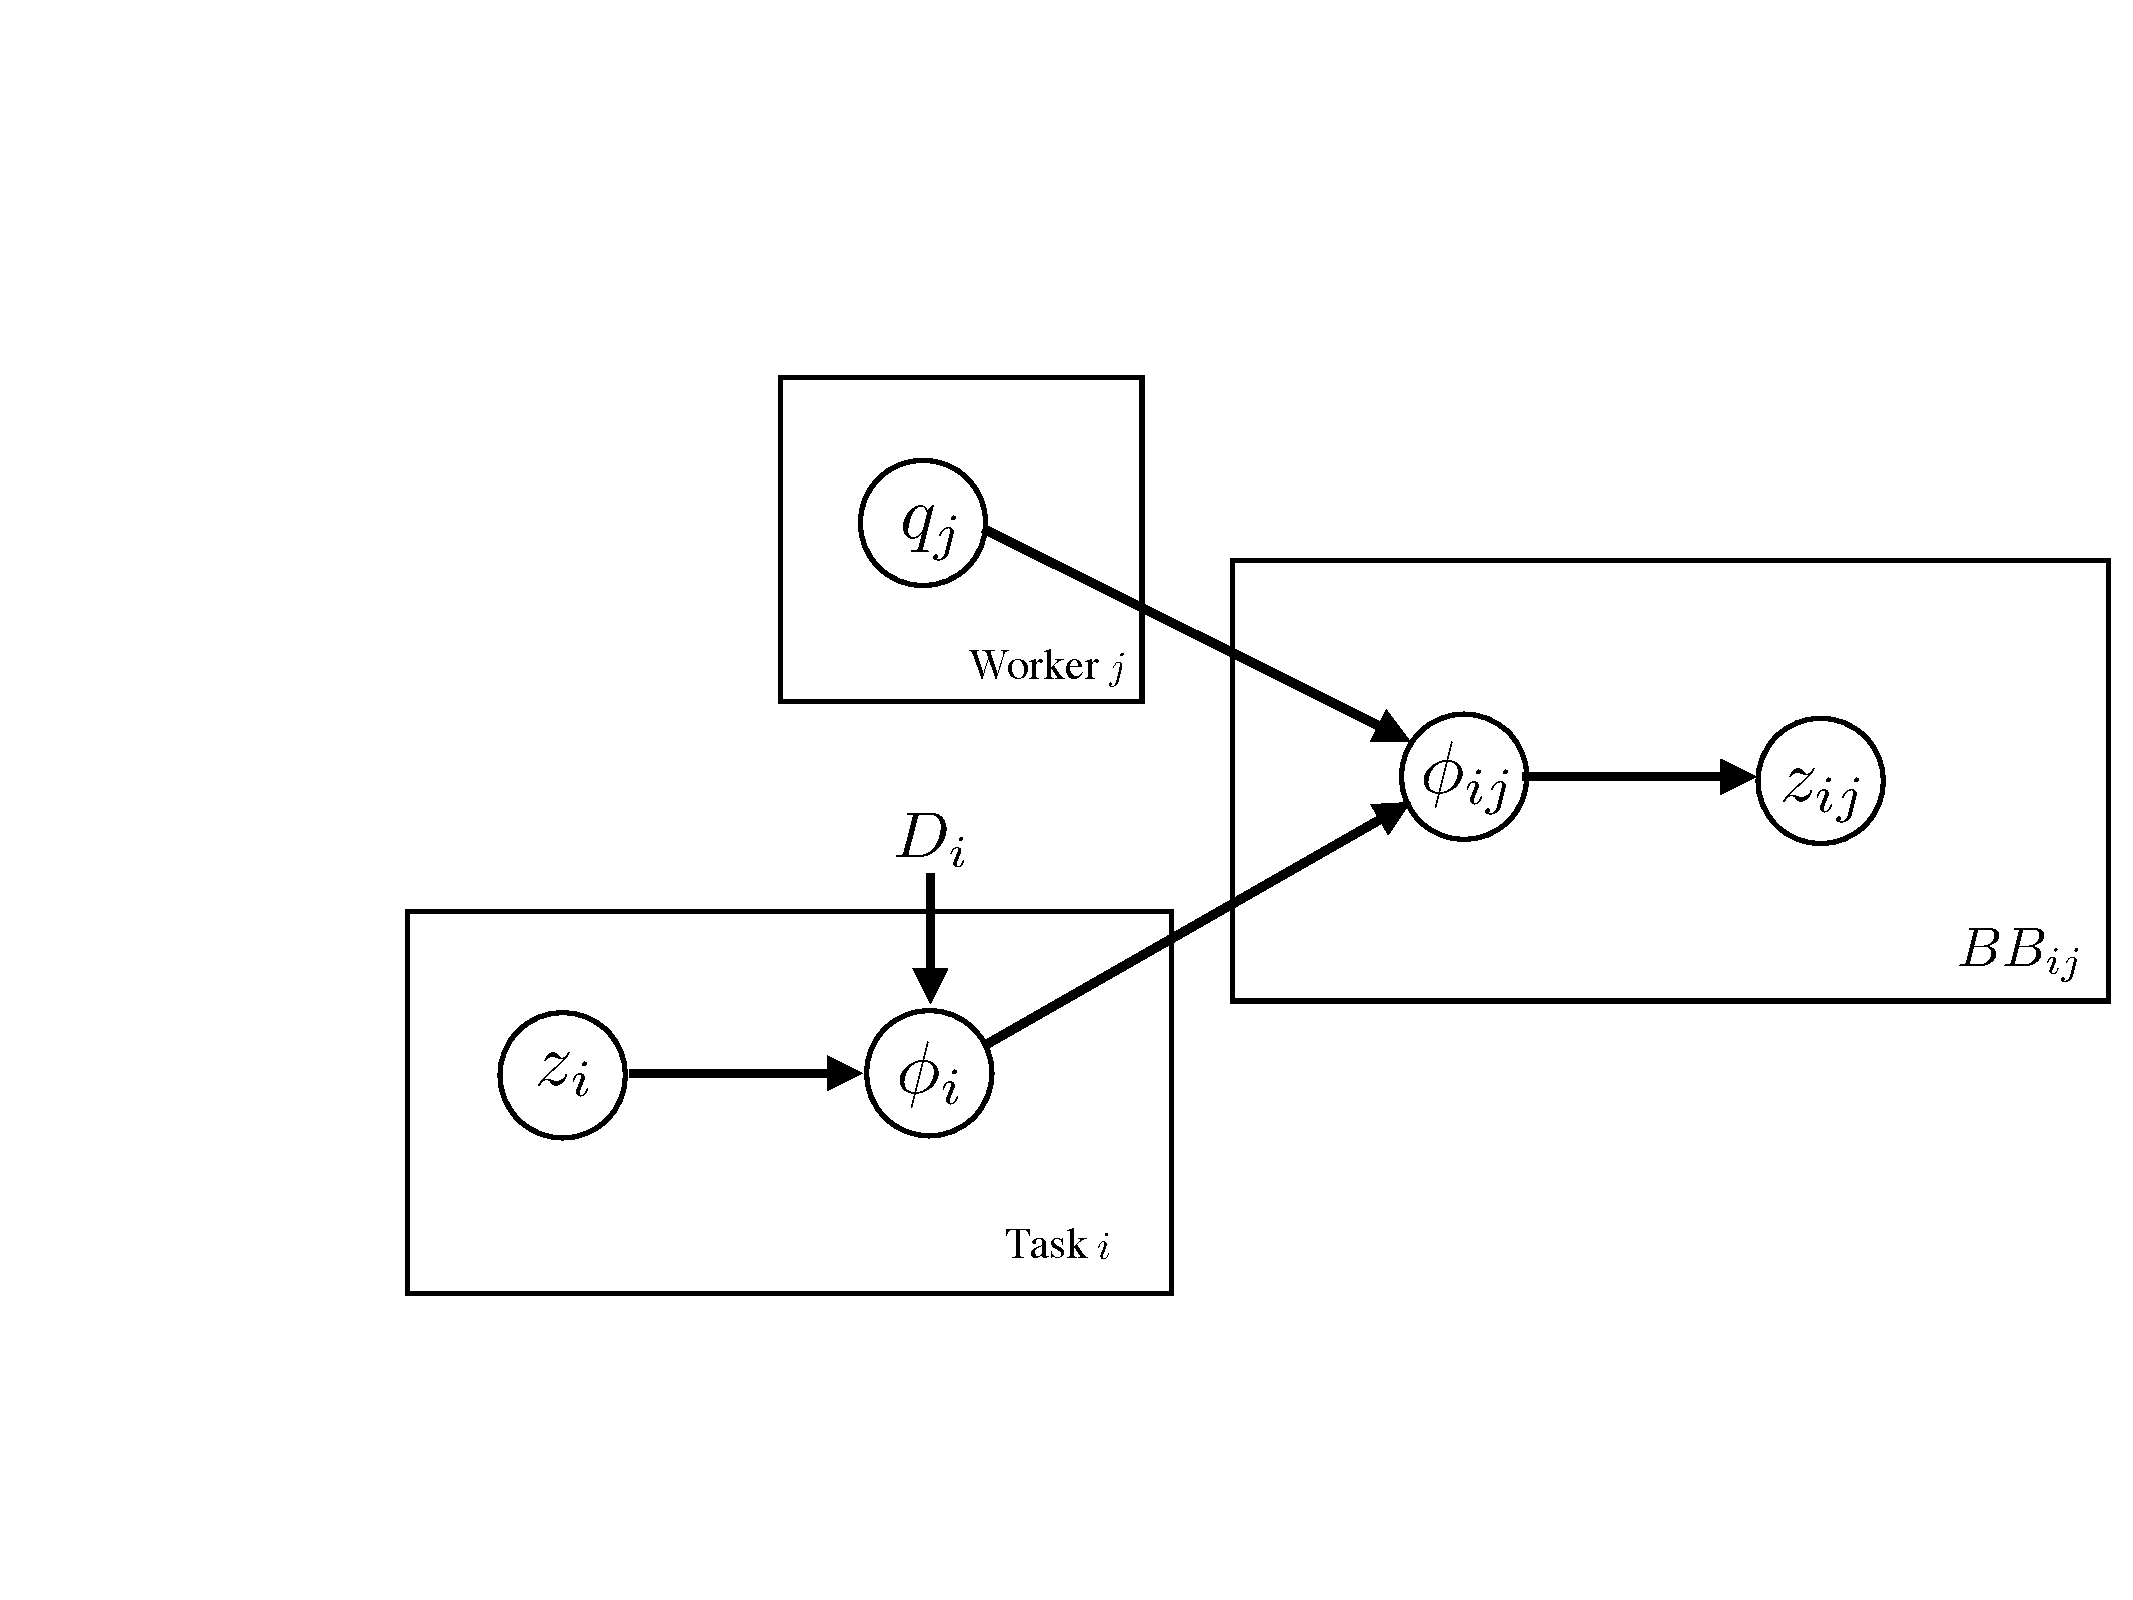
\includegraphics[trim=1cm 5cm 1cm 5cm,width=0.8\linewidth]{plots/generative_pgm.pdf}
\caption{Proposed probabilistic graphical model for crowdsourcing image segmentation.}
\end{figure}
The generative model is inspired by \cite{Welinder2010}, the process is as follows:
\begin{itemize}
\item A task is defined by an object-image pair i : 
\begin{itemize}
\item $z_i$ is hidden variable that completely describes the ground truth BB from the image (e.g. set of all points in $BB_G$).
\item  $\phi_j$ is some descriptive image-related quantity extracted from $BB_G$ This can either be a 1-D scalar aggregate or a multidimensional quantity. (e.g. boundary complexity of the image boundary)
\item $J_i$ is the set of all workers j that annotated the object-image. 
\item $D_i$ is the task difficulty of object-image i.  The $\phi_i$ image summary is determined by both the objective description of $BB_G$ ($z_i$) and the difficulty of the task. The task difficulty is a measure of how far off are most of the worker's responses compared to $BB_G$.  
\begin{equation}
D_i = \sum_{j\in J_i} dist(\phi_j,\phi_i)
\end{equation}
Here, we can model the distribution of $\phi_i$ as :
$$p(\phi_i|z_i) = N(\phi_i;z_i,D_i^2)$$
This agrees with our intuition that in a distribution of image descriptions for all workers, the larger the spread means that the task is difficult. The distribution is centered around $z_i$ (i.e. complete description of $BB_G$).
\end{itemize}
\item By definition, we assume here that task difficulty is completely a result of the image itself and independent of any worker qualities. $q_{ij}$ is the quality of worker j for object i evaluated against $BB_{G,i}$. We can also try to model user expertise, but this is less important in salient, common-object segmentation. If we chose to take the prior appraoch, we assume that $q_{ij}$ only parameterizes the vision-related quantities affecting worker j's judgement on $\phi_{ij}$.
\begin{equation}
q_{ij} = dist(\phi_{ij},\phi_i)
\end{equation}
\item Both the characteristics of the ground truth BB ($\phi_i$) and the worker's ability to segment the image ($q_i$) would determine how the worker would percieve the image($\phi_{ij}$) and what worker's BB would look like ($z_{ij}$).
%\item Finally, the characteristics of the BB drawn by worker i is just a summary of the BB drawn by worker i ($BB_i$)
\end{itemize}
\section{Metrics for $\Phi$ Functions}
\par There are two sets of annotations that we used as ground truth comparison for computing these metrics: gold-standard annotations cross-matched with MSCOCO (\texttt{[COCO]}) and detailed annotation boundaries drawn by me with the same web interface (\texttt{[Self]}). Note that some of the COCO annotations lack exact cross matches. The metrics computed for objects that are not in the COCO database are flagged and not used for computing the evaluation metrics. However, inexact annotations of the same object (e.g. book-labeled object with only book cover annotation) is still incorporated in the computed metrics. The evaluation metrics can be grouped into three categories: 
\paragraph{Area-based: } These methods include precision, recall, area ratio or boundary complexity. 
\begin{align}
\texttt{Precision} = \frac{area(BB_i\cup T)}{area(T)} \\
\texttt{Recall} = \frac{area(BB_i\cup T)}{area(BB_i)} \\
\texttt{Jaccard} = \frac{area(BB_i\cap T)}{area(BB_i \cup T)}
\end{align}
Area ratio is a simple baseline proposed by  \cite{Vittayakorn2011} based on the intuition that larger objects should be easier to annotate than smaller objects, so larger annotations should be better than smaller ones.
\begin{equation}
\texttt{Area ratio}=\frac{area(BB_i)}{\text{Total image area}}
\end{equation}
\paragraph{Boundary-based:} \par While precision, recall, and majority-vote are simple metrics, since they are bounded by [0,1], metrics computed against BBG should always be 1. In addition these projection functions do not capture the full resolution of the bounding box.  
\par \cite{Vittayakorn2011} proposes a bipartite-matching measure based on the Euclidean distance between two BBs. First, they randomly sample m=300 points along the annotation boundary, then compute all pairwise Euclidean distance. Then, the Kuhn-Munkres algorithm is used to match together the orientation of the two annotations, and returns the assignments that yields the minimum Euclidean. Finally, the normalized score ($\texttt{NME}$) of an annotation i is computed as:
\begin{equation}
score = 1-\frac{dist_i}{max(dist)}
\end{equation} where max(dist) is the maximum Euclidean distance of all the annotations computed in our dataset. Our implementation differs slightly in that we conduct a B-spline parametric interpolation of use m=50 points along the boundary rather than random sampling, in order to speed up the computation in the Munkres algorithm. These implementation details should have little effect on the Euclidean scores computed.
\par  Another simple baseline used by \cite{Vittayakorn2011} is simple a unnormalized count of the number of control points in a user's annotation (\texttt{Num Points}), based on the intuition that a more carefully-annotated would result in a better annotation. Since some objects may have inherently simple geometries that could be well-annotated with a small number of control point, to account for the object's boundary complexity, one possible derived measure could be to normalize by the max number of control point) of the particular object.\footnote{Since this is a constant for each object i, it would not affect the form of the $J_i$ distribution.} 
\paragraph{Contrast-based: } These methods examine how close is BB to regions of contrasts detected by CV algorithms (saliency maps, Bayesian Matting) or edge detectors. A major problem when implementing these methods is group and match CV regions to BB annotations, since CV methods often yield over-segmented regions.
\section{Preliminary Experiment}
We ran a preliminary experiment where each HIT consisted of one annotation task for a specific pre-labelled object in the image, as shown in Fig.\ref{interface}. There is a total of 46 objects in 9 images from the MSCOCO dataset\cite{Lin2014}. These objects and images are intentionally chosen so that they represent a variety of image difficulty (based on object clutter-ness) and potential logical error and level of ambiguity. The average number of objects annotations that each worker completed was 10.16. The average time to complete each HIT is 83.96 seconds and workers are compensated for 5 cents per HIT.  For each object, we collected annotations from a total of 40 independent workers.
\subsection{Data Observations}
\begin{itemize}
\item \textbf{Basic statistical summary:}
Most workers makes decent annotation that closely follows the ground-truth BB, since the mean is close to one and standard deviation is large for most metrics.  The annotations with metric scores significantly below a threshold are likely mistakes due to task ambiguity and ground-truth mismatches, as we can see that applying work quality filter significantly improves the mean and SD.
\begin{table}[h]
\centering
\begin{tabular}{lrr}
\hline
 All              &   Mean &     SD \\
\hline
 Precision [COCO] &  0.87  &  0.22  \\
 Recall [COCO]    &  0.9   &  0.12  \\
 Jaccard [COCO]   &  0.79  &  0.22  \\
 NME [COCO]       &  0.94  &  0.12  \\
 Num Points       & 26     & 19     \\
 Precision [Self] &  0.86  &  0.21  \\
 Recall [Self]    &  0.9   &  0.14  \\
 Jaccard [Self]   &  0.78  &  0.22  \\
 NME [Self]       &  0.94  &  0.13  \\
 Area Ratio       &  0.063 &  0.089 \\
\hline
\end{tabular}
\begin{tabular}{lrr}
\hline
 Filter\ensuremath{>}0.6       &   Mean &     SD \\
\hline
 Precision [COCO] &  0.93  &  0.069 \\
 Recall [COCO]    &  0.92  &  0.072 \\
 Jaccard [COCO]   &  0.86  &  0.084 \\
 NME [COCO]       &  0.96  &  0.055 \\
 Num Points       & 26     & 19     \\
 Precision [Self] &  0.92  &  0.076 \\
 Recall [Self]    &  0.93  &  0.074 \\
 Jaccard [Self]   &  0.86  &  0.086 \\
 NME [Self]       &  0.96  &  0.053 \\
 Area Ratio       &  0.063 &  0.089 \\
\hline
\end{tabular}
\caption{Left: Statistics for all workers; Right: for good workers only [metric$\geq$0.6]}
\label{basic_stat}
\end{table}
\item Both the number of tasks each worker takes on and average time in a task follows a Pareto-like, long-tail distribution, which is typical for crowdsourcing applications.
\item \textbf{Data Fitting Procedure:} We are interested in figuring out what functional form these $\Phi$ functions are distributed as. We fitted the histograms against 84 different probability distribution functions\footnote{Most of the functions in  \href{https://docs.scipy.org/doc/scipy/reference/stats.html}{scipy.stats}:\tiny{[alpha, anglit, arcsine, beta, betaprime, bradford, burr, cauchy, chi, chi2, cosine, dgamma, dweibull, expon, exponpow, exponweib, f, fatiguelife, fisk, foldcauchy, foldnorm, frechet\_l, frechet\_r, gamma, gausshyper, genexpon, genextreme, gengamma, genhalflogistic, genlogistic, genpareto, gilbrat, gompertz, gumbel\_l, gumbel\_r, halfcauchy, halflogistic, halfnorm, hypsecant, invgamma, invgauss, invweibull, johnsonsb, johnsonsu, ksone, kstwobign, laplace, levy, levy\_l, loggamma, logistic, loglaplace, lognorm, lomax, maxwell, mielke, nakagami, ncf, nct, ncx2, norm, pareto, pearson3, powerlaw, powerlognorm, powernorm, rayleigh, rdist, recipinvgauss, reciprocal, rice, semicircular, t, triang, truncexpon, truncnorm, tukeylambda, uniform, vonmises, vonmises\_line, wald, weibull\_max, weibull\_min, wrapcauchy]}}, using the maximum-likelihood estimators of these distributions. Then, a  Kolmogorov-Smirnov test  assessed the statistical significance of whether the fitted function and the data follow the same distribution. We quantify the best fits using minimal residual sum-of-square (RSS) and the p-value resulting from the KS-test.  To preserve the tails of these distributions, no filtering for selecting good workers only was done in the fitting procedure. 
\end{itemize}
\subsection{Overall Distribution}
\begin{figure}[ht]
\centering
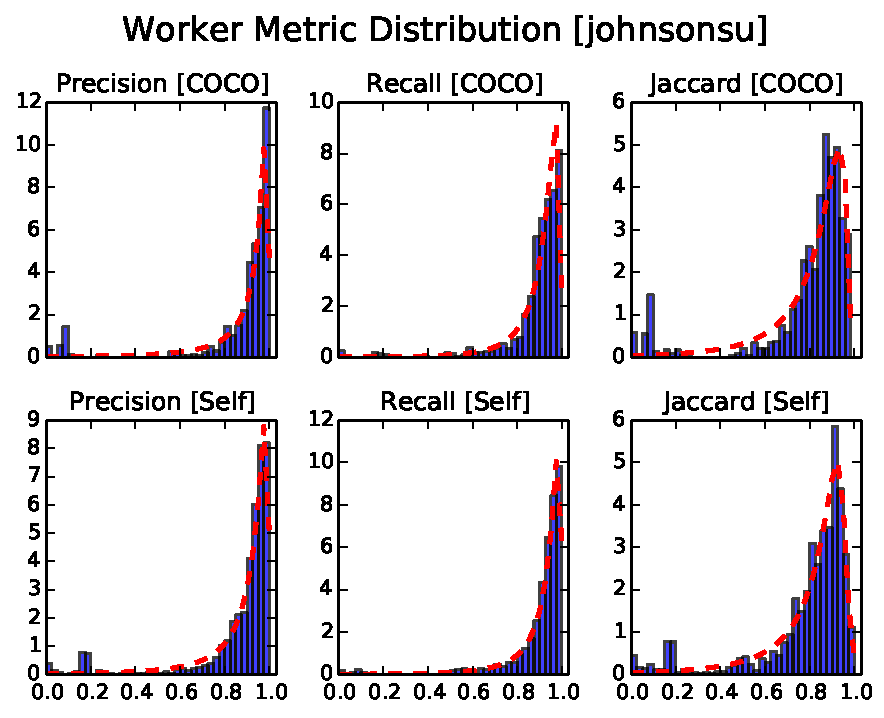
\includegraphics[width=\linewidth]{plots/johnsonsu_fitted_metric_histogram.pdf}
\caption{Normalized histogram of metric values, fitted with a Johnson SU distribution. }
\label{metric_hist}
\end{figure}
\par Overall distribution contains each of the metrics computed from all tasks submitted by all workers (N=1947). The histogram distribution (fixed bin size =50) of these metrics resembles a long-tail, exponential-decaying distribution. As shown in the best-fitting functions in Table \ref{overall_best_fits}, there are many pdfs that fits one metric but not another. 
\par One particular distribution that yields the best fits for many metrics is the Johnson unbounded (SU) distribution, which we summarized in Table \ref{jsu_tbl}. The Johnson SU distribution is a transformed Gaussian where the data $x\mapsto\gamma+\sigma \sinh^{-1}(\frac{x-\xi}{\lambda})$, which effectively maps the typical two-parameter Gaussian to a more flexible, four parameter pdf to better account for the skewness (heavily right-skewed) and kurtosis (long-tail) of the distribution.
%\subsubsection{Testing Assumption 2: }
%Since our metrics are all 
%ground truth means that --- as 1. So effectively, we are measuring 1-f(x) 

%\item We are interested in whether our data agrees with Assumption \#2 and \#3 regarding work quality and task difficulty. 
%If a worker's response differs greatly from the ground truth, then work quality ($Q_w$) is low. 
%If many of the worker's response differs greatly from ground truth for a particular image, then task difficulty ($D_t$) is high.

\subsection{Object-level Distributions}
\par Recall that $J_i$  is the set of all workers j that annotated the object-image i, we are interested in finding out how these workers are distributed in order to deduce worker quality. 
\par In the data fitting procedure, the bin size is an important hyperparameter. When the bin size is small, the histogram is very smoothed, so many different functional forms can be fitted. Since our data is N=40, we pick a bin size of 30. Due to the large number of $J_i$ distributions, we conducted the fitting procedure on a smaller candidate set of more interpretable functional forms\footnote{Based on our overall function fitting results: Gaussian, Johnson SU/SB, Cauchy, Beta, Loggamma, generalized gamma, Gompertz and t-distributions}.
\par  Table \ref{all_Ji_fit} summarizes the best functional fit for each metric, based on the average RSS across all $J_i$ distributions. The magnitude of RSS for the fitted function of each metric is very different. If we examine a rankings, the RSS difference between the top few best-fit functions is minimal and usually contain the Johnson SU distribution, so the Johnson SU distribution is a sufficiently good description of these $\Phi$ metrics. 
%\par Many of the best-fitting functional form of $\Phi$ in Table \ref{all_Ji_fit} may make the inference problem challenging. While the Gaussian does not yield the best fit, it is a more interpretable $\Phi$ function and may be easier for inference. Some of the non-Gaussianity may also be due to the small sample size in our preliminary experiment (N$\approx$40 for each $J_i$ distribution). We are interested in assessing whether it can be a ``good-enough'' fit based on RSS. 
%\par  Fig.\ref{GaussRSSBox} shows a boxplot of the RSS based on the Gaussian fits for all the $J_i$ distributions. We could see that the number of control points have several orders of magnitude lower RSS than other metrics. This makes sense because \texttt{Num Points} is the only metric that measures \textit{only} how carefully drawn the BB is, which would in theory match with a spread in worker dexterity. All other metrics (except \texttt{Area Ratio}) are confounded by potential BB mismatch or task ambiguity mistakes because of normalization or comparison against a gold standard BB. 
%\begin{figure}[ht]
%\centering
%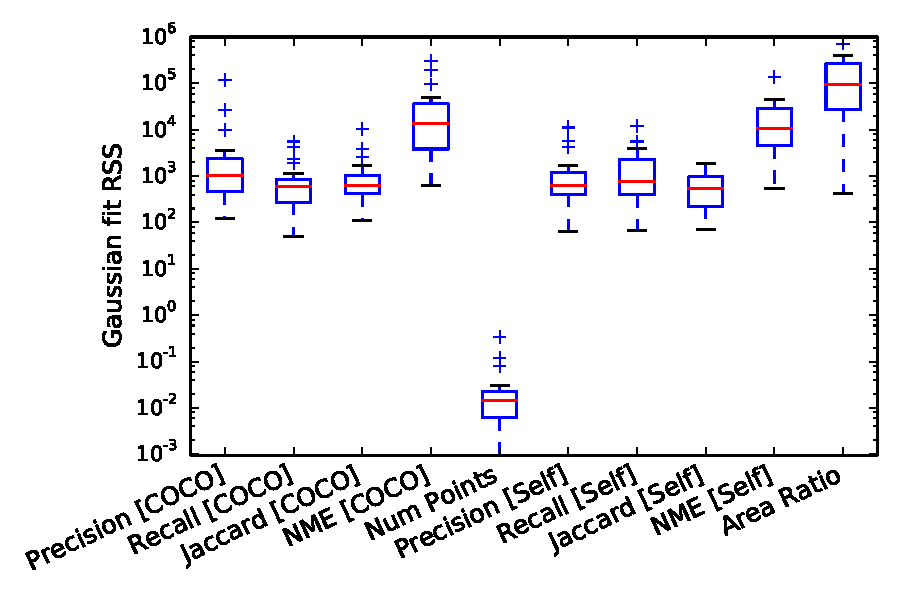
\includegraphics[width=0.6\linewidth]{plots/GaussianRSSBoxplot.pdf}
%\caption{The boxplot shows the spread of RSS for all $J_i$ distribution based on Gaussian fits.}
%\label{GaussRSSBox}
%\end{figure}
%\subsubsection{Testing Assumption 3: Influence of task difficulty on spread}
%We are interested in testing our hypothesis that if work quality exhibits a large spread, that means that the object i is probably very hard to annotate. If we exclude difficult task due to task ambiguity, we hypothesize that the number of points in the image object (as a measure of boundary complexity) should depend on the standard deviation of the fitted distribution (Gaussian or Johnson SU). As summarized in Table \ref{assum3}, the Pearson's test shows that there is \textit{very little evidence for linear correlation} between the number of points in an object and the standard deviation of the fitted function. One potential reason for this is that the number of points is not a good metric of task difficulty, since we know that there are other types of error that could make a task difficult (small object area and task ambiguity) A potential next step would be to look at how the data for selected object subpopulations that are prone to each errors type would behave, but due to the small number of objects in each category the results for this analysis will probably not be very generalizable. 
\bibliographystyle{plain}
\bibliography{reference}

\newpage
\begin{appendices}
\section{Best-fit summaries}
\begin{table}[ht]
\centering
\begin{tabular}{llrrr}
\hline
 metric           & Function Name   &       RSS &   D-value &   p-value \\
\hline
 Precision [COCO] & beta            &  9.11     &      0.48 &  1.02e-05 \\
 Recall [COCO]    & loggamma        &  4.56     &      0.46 &  2.76e-05 \\
 Jaccard [COCO]   & gompertz        & 13.3      &      0.46 &  2.76e-05 \\
 NME [COCO]       & cauchy          & 51.7      &      0.84 &  1.25e-16 \\
 Num Points       & johnsonsb       &  0.000239 &      1    &  2.16e-23 \\
 Precision [Self] & johnsonsu       &  6.02     &      0.34 &  0.00443  \\
 Recall [Self]    & johnsonsu       &  5.07     &      0.42 &  0.000178 \\
 Jaccard [Self]   & johnsonsu       &  4.57     &      0.28 &  0.0317   \\
 NME [Self]       & johnsonsb       & 30.3      &      0.74 &  5.31e-13 \\
 Area Ratio       & gengamma        & 27.1      &      0.34 &  0.00443  \\
\hline
\end{tabular}
\caption{Shapewise, the RSS is a better measure of functional fit than p-value, so we use this for evaluating the best-fitting pdf for each measure. This table summarizes the best-fitting function for each metric.}
\label{overall_best_fits}
\end{table}

\begin{table}[ht]
\centering
\begin{tabular}{lrrrrrrr}
\hline
 metric           &      RSS &   D-value &   p-value &   $\xi$ &   $\lambda$ &   Shift &   Scale \\
\hline
 Precision [COCO] & 10       &      0.36 &   0.0021  &  5.2 &     0.75 &  1      & 0.00011 \\
 Recall [COCO]    &  7       &      0.44 &   7.2e-05 &  5.9 &     1.1  &  1      & 0.00062 \\
 Jaccard [COCO]   & 14       &      0.3  &   0.017   &  5.6 &     1.1  &  0.99   & 0.0017  \\
 NME [COCO]       &  2.2e+02 &      0.7  &   1.1e-11 &  1.3 &     0.61 &  0.99   & 0.0032  \\
 Num Points       &  0.00044 &      1    &   2.2e-23 & -6.2 &     1.2  &  0.8    & 0.21    \\
 Precision [Self] &  6.8     &      0.34 &   0.0044  &  5.6 &     0.84 &  1      & 0.00018 \\
 Recall [Self]    &  5.5     &      0.42 &   0.00018 &  5.5 &     0.91 &  1      & 0.00029 \\
 Jaccard [Self]   &  4.6     &      0.28 &   0.032   &  1.6 &     0.95 &  0.96   & 0.039   \\
 NME [Self]       &  1.1e+02 &      0.64 &   7.8e-10 &  1.2 &     0.61 &  0.99   & 0.0037  \\
 Area Ratio       & 30       &      0.32 &   0.0089  & -4.9 &     0.78 & -0.0002 & 0.00012 \\
\hline
\end{tabular}
\caption{Johnson SU fitting coefficients.}
\label{jsu_tbl}
\end{table}

\begin{table}[ht]
\centering
\begin{tabular}{llr}
\hline
 metric           & Function   &       RSS \\
\hline
 Area Ratio       & johnsonsu  & 273751.49 \\
 Jaccard [COCO]   & johnsonsu  &    675.65 \\
 Jaccard [Self]   & cauchy     &    250.42 \\
 NME [COCO]       & johnsonsu  &  27439.87 \\
 NME [Self]       & johnsonsu  &  10812.98 \\
 Num Points       & cauchy     &      0.06 \\
 Precision [COCO] & johnsonsu  &   4570.24 \\
 Precision [Self] & johnsonsu  &   1414.98 \\
 Recall [COCO]    & johnsonsu  &    452.79 \\
 Recall [Self]    & beta       &    902.61 \\
\hline
\end{tabular}
\caption{Best functional fit for each metric, as determined by average RSS across all objects in the $J_i$ distribution.}
\label{all_Ji_fit}
\end{table}
\begin{table}[ht]
\centering
\begin{tabular}{lrrrrrrrrrr}
\hline
          &   P [C] &   R [C] &   J [C] &   NME [C] &   NumPt &   P [C] &   R [S] &   J [S] &   NME [S] &   Area \\
\hline
 R [Norm] &    0.05 &   -0.27 &   -0.11 &      0.32 &    0.84 &    0.18 &   -0.36 &   -0.05 &      0.27 &   0.60 \\
 p[Norm]  &    0.85 &    0.30 &    0.67 &      0.22 &    0.00 &    0.49 &    0.15 &    0.87 &      0.29 &   0.01 \\
 R [JSU]  &    0.31 &    0.02 &    0.03 &     -0.12 &   -0.26 &    0.47 &   -0.19 &    0.61 &      0.51 &   0.27 \\
 p [JSU]  &    0.22 &    0.95 &    0.90 &      0.64 &    0.31 &    0.05 &    0.47 &    0.01 &      0.04 &   0.29 \\
\hline
\end{tabular}
\caption{Pearson's linear correlation coefficient when comparing the average number of points in BB drawn by all worker(as an indicator for task difficulty) and the standard deviation of the worker distribution (against \texttt{JSU} and \texttt{Norm} distributions). [C],[S] short for [COCO] and [Self].}
\label{assum3}
\end{table}

\newpage
\section{Data Examples}
\begin{figure}[ht!]
\centering
\fbox{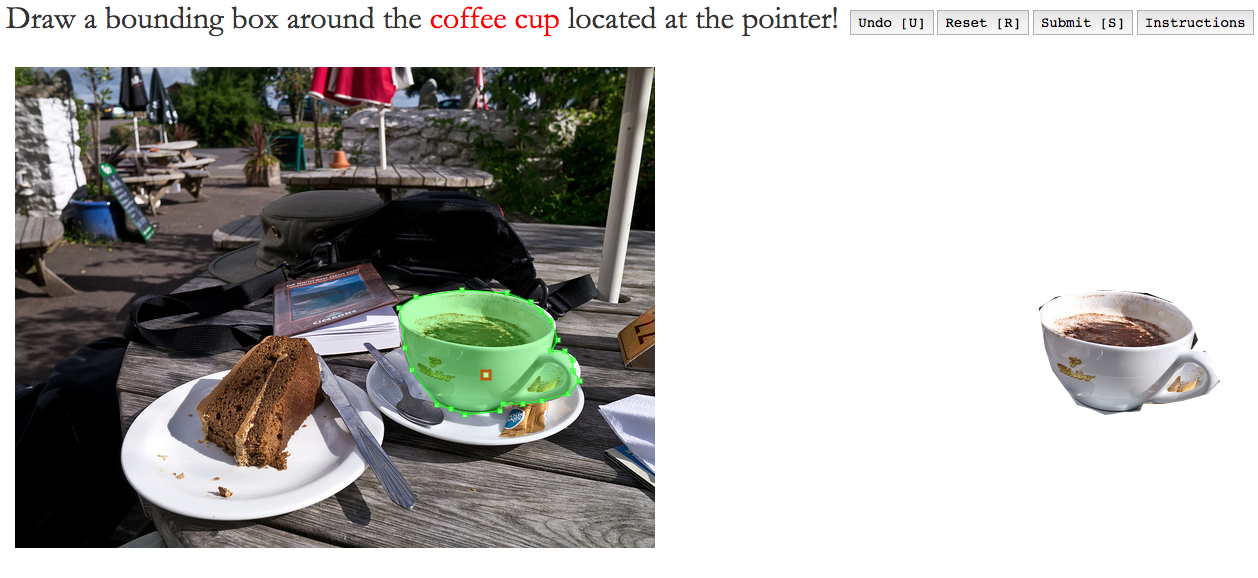
\includegraphics[width=0.9\linewidth]{plots/interface.png}}
\caption{An example interface for the segmentation webapp can be seen  \href{http://crowd-segment.herokuapp.com/segment/COCO_train2014_000000000127/10/}{here}.}
\label{interface}
\end{figure}
Visualizations for all the object annotations could be found \href{http://nbviewer.jupyter.org/github/dorisjlee/crowd-seg/blob/master/analysis/2017_01_16_Visualize_all_bb_results.ipynb}{here}.
\begin{figure}[ht]
\centering
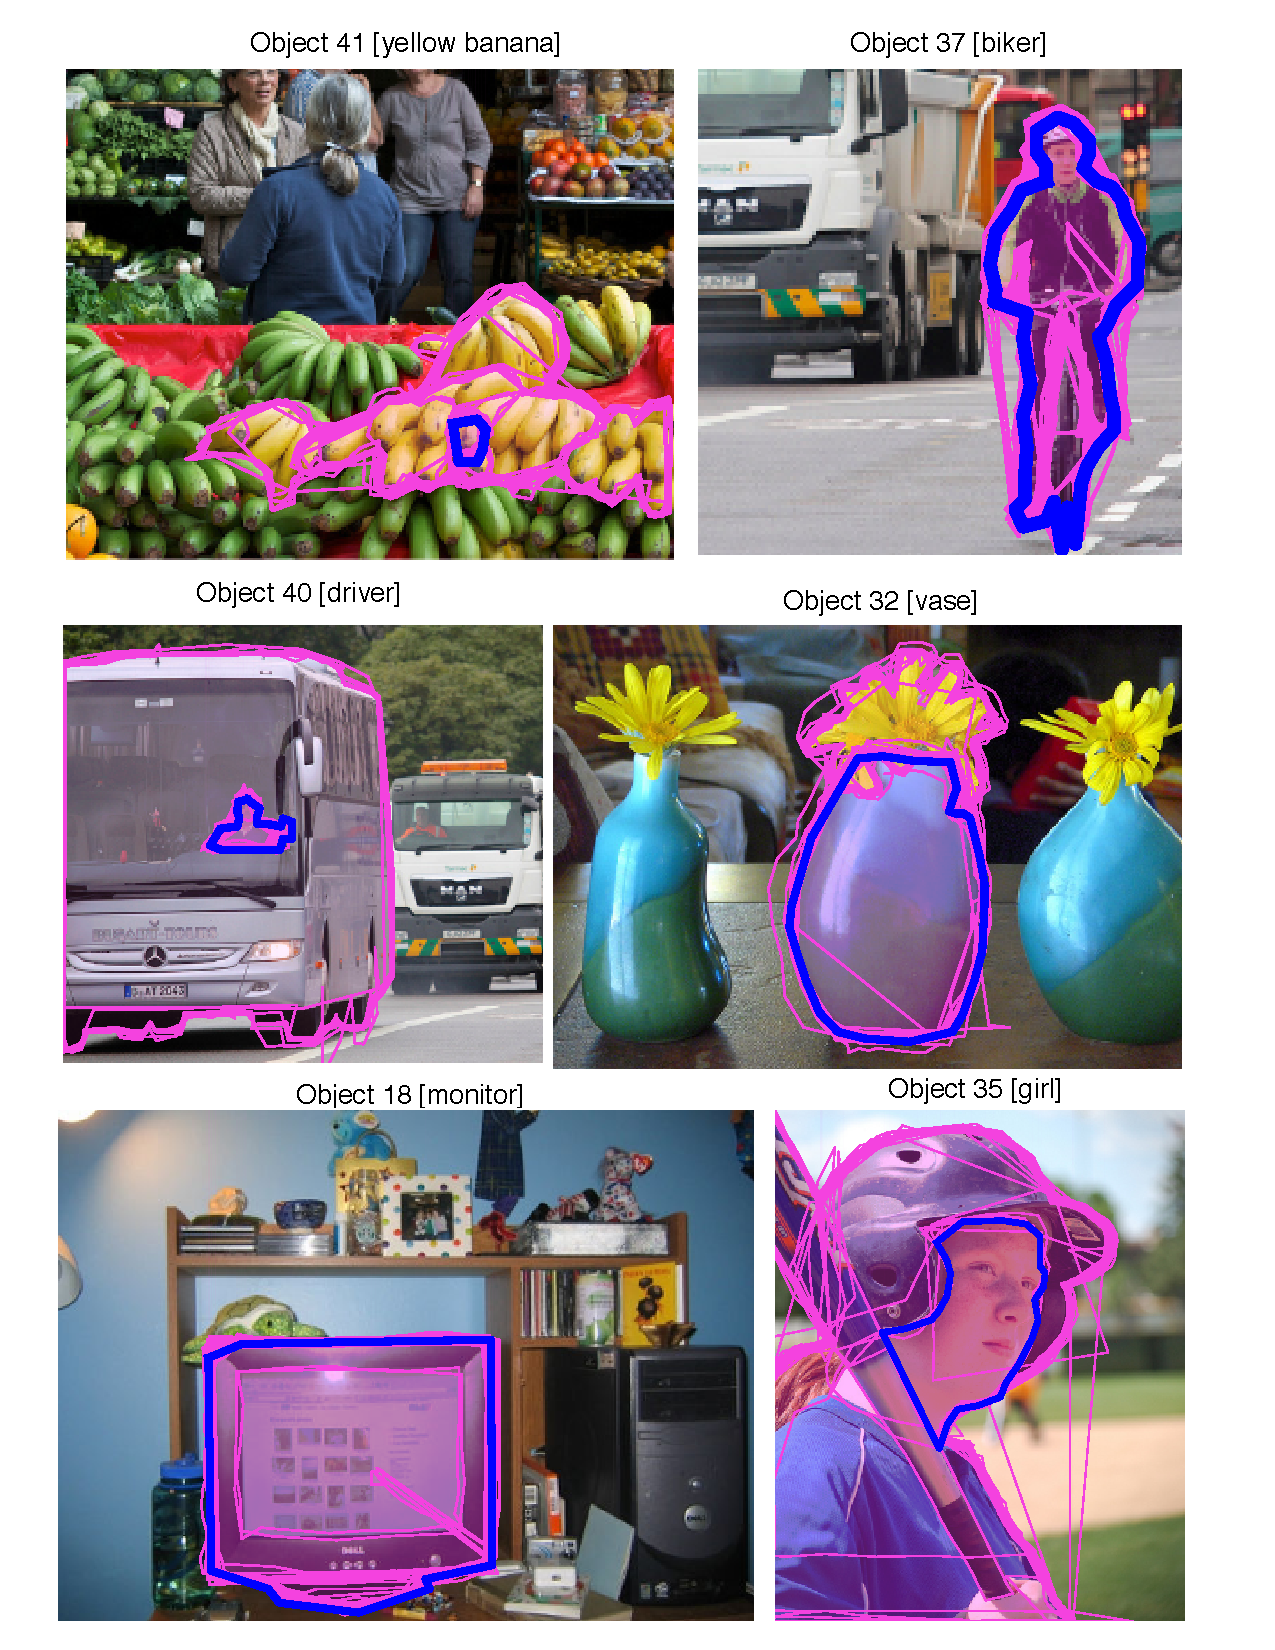
\includegraphics[width=\linewidth]{plots/task_ambiguous_cases.pdf}
\caption{Selected task ambiguous object that is exlucded in the task difficulty analysis. }
\end{figure}

\end{appendices}
\end{document}
